Large language models can generate structured outputs, but their reliability often depends on how the task is presented to them. Prompt engineering has therefore become a central technique. By carefully designing instructions, examples, and schema descriptions in the prompt, users can guide LLMs to align their generative outputs with the structured requirements of template filling.

The idea that LLMs can adapt to new tasks without retraining was first demonstrated through in-context learning. Brown et al.\ showed that GPT-3 could perform unseen tasks when given only a natural language description and a few examples \cite{brown2020language}. Later studies such as Wei et al.\ explored the so-called “emergent abilities” of LLMs, where models suddenly demonstrate strong zero-shot and few-shot performance once they reach a certain scale \cite{wei2022emergent}. For information extraction, this means that a model can often fill structured fields if the prompt specifies the task and provides one or two demonstrations.

Designing effective prompts, however, is not straightforward. Sun et al.\ \cite{sun2023slot} propose structured prompts for speech-based slot filling that include task definitions, slot descriptions, and linearized external knowledge. Their experiments show that such prompt structures make LLMs more robust to noise in automatic speech recognition (ASR) transcripts. Similarly, Lin et al.\ \cite{lin2021leveraging} show that including slot descriptions directly in prompts improves zero-shot dialogue state tracking, since it grounds the model in the meaning of each field. These studies highlight how prompts can embed domain knowledge and ontology definitions to improve extraction quality.

The choice between zero-shot and few-shot prompting also affects performance. Zero-shot prompts rely only on schema descriptions, which makes them flexible but often less reliable. Few-shot prompting, where carefully selected input–output examples are added to the prompt, improves consistency but comes at the cost of longer prompts and higher inference latency. Pan et al.\ \cite{pan2023chatgpt} evaluated ChatGPT for dialogue understanding and found that few-shot prompting consistently outperformed zero-shot in accuracy, though response times increased.

\begin{figure}
    \centering
    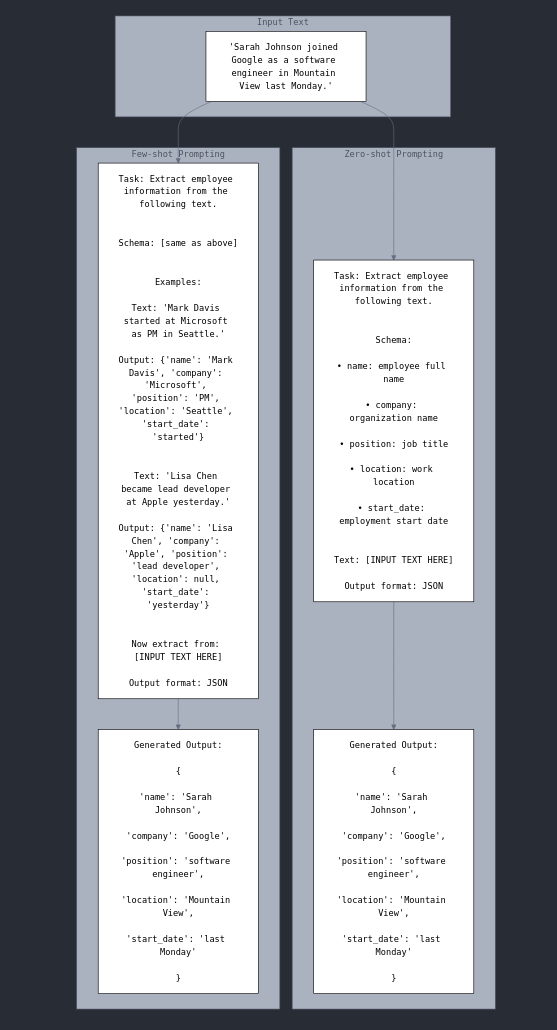
\includegraphics[width=0.8\linewidth]{images/zero_shot_vs_few_shot.png}
    \caption{Zero-shot vs Few-shot Prompting for Template Filling}
    \label{fig:placeholder}
\end{figure}

Schema-constrained prompting has also been investigated as a way to enforce output structure. Zhang et al.\ \cite{zhang2023sgptod} introduced SGP-TOD, where prompts embed schema definitions for task-oriented dialogue systems. By instructing the model to generate only values that fit the schema, they reduced invalid or inconsistent outputs. Practical systems follow the same idea: Google’s LangExtract \cite{google2024langextract} lets users define a JSON schema and then generates extractions that are automatically validated against it. While this approach provides consistency in output format, it remains monolithic and does not allow modular correction or multi-model validation.

Beyond hand-crafted design, some studies explore automated prompt optimization. Peng et al.\ \cite{peng2023check} propose a framework where candidate prompts are iteratively refined based on feedback signals, such as factual errors or schema mismatches. This “prompt tuning without training” approach suggests that prompts themselves can be systematically improved using evaluation signals, rather than relying only on human intuition.

In summary, prompt engineering has proven to be a powerful tool for adapting LLMs to information extraction tasks. It enables zero-shot and few-shot template filling, allows domain knowledge to be embedded into prompts, and supports schema-constrained generation. At the same time, it has clear limitations: prompts are often brittle, performance varies with phrasing, and external validation is still needed to ensure correctness. These weaknesses motivate research into more modular and interactive systems, where prompt design is combined with additional layers of control. The next subsection therefore examines multi-agent LLM systems, which distribute responsibilities across specialized agents to improve transparency, adaptability, and correction.
